% Architecture -- paper plan Task 2.
% TikZ diagram of the pipeline AS IMPLEMENTED (prototype/healgen/*):
% draft-first decomposition, sufficiency-gated retrieval, DCEG, localized repair, confidence composer.

\section{Architecture}
\label{sec:architecture}

\subsection{Conceptual Overview and Analogy}
Large language models generate responses sequentially by sampling tokens from a conditional probability distribution. While this produces fluent prose, it lacks an explicit factual verification mechanism: a model can assert speculative or incorrect facts with equal confidence. Existing solutions typically follow one of two extremes: \emph{always-on pre-retrieval} (standard RAG), which queries an external database for every prompt before generation, or \emph{monolithic post-hoc editing} (such as CoVe \cite{dhuliawala2023cove}), which rewrites the entire response after generation.

HealGen introduces a \textbf{draft-first, claim-level self-healing architecture}. To understand the intuition, consider how an experienced researcher drafts a report:
\begin{enumerate}
  \item \textbf{Draft first:} The writer produces an initial draft directly from memory without interrupting their flow of reasoning.
  \item \textbf{Decompose assertions:} The writer reviews what was written, breaking complex sentences into individual, bite-sized factual claims.
  \item \textbf{Check sufficiency on demand:} For each claim, the writer evaluates whether their current reference notes already contain sufficient proof. If proof is missing, they perform a targeted reference lookup.
  \item \textbf{Graph grounding:} The writer builds a mental map linking each assertion to its supporting evidence, highlighting unsupported or contradictory claims.
  \item \textbf{Surgical repair:} Rather than discarding and rewriting the entire draft, the writer surgically edits \emph{only the specific sentences} containing unsupported claims, leaving all verified sentences 100\% byte-identical.
\end{enumerate}

Figure~\ref{fig:pipeline} illustrates this closed inference loop as implemented in our open prototype (\texttt{prototype/healgen/*}), organized into three functional stages.

\begin{figure*}[t]
\centering
\begin{tikzpicture}[
    font=\sffamily\footnotesize,
    >=Stealth,
    stage/.style={
        draw=#1!75!black, fill=#1!8, rounded corners=3.5pt, line width=0.8pt,
        align=center, minimum height=10mm, inner xsep=5pt, inner ysep=4pt,
        font=\sffamily\scriptsize
    },
    stage/.default=blue,
    cond/.style={
        draw=orange!85!black, fill=orange!10, rounded corners=3.5pt, line width=0.9pt,
        align=center, minimum height=10mm, inner xsep=5pt, inner ysep=4pt,
        font=\sffamily\scriptsize
    },
    groupbox/.style={
        draw=#1!45, fill=#1!3, rounded corners=5pt, line width=0.65pt, dashed
    },
    grouplabel/.style={
        font=\sffamily\bfseries\tiny, text=#1!85!black, anchor=north west, xshift=5pt, yshift=-3pt
    },
    arrow/.style={->, line width=1.0pt, draw=gray!80!black},
    dedge/.style={->, dashed, line width=1.0pt, draw=teal!80!black},
    stepbadge/.style={
        circle, fill=#1!85!black, text=white, font=\sffamily\bfseries\tiny,
        inner sep=0.8pt, minimum size=11pt
    },
    stepbadge/.default=blue,
    callout/.style={
        draw=teal!70!black, fill=teal!6, rounded corners=3.5pt, line width=0.65pt,
        font=\sffamily\scriptsize, align=left, inner sep=4.5pt
    }
]

  % -------------------------------------------------------------
  % Top Row: Forward Evaluation & Retrieval
  % -------------------------------------------------------------
  \node[stage=blue] (draft) {
    \textbf{Draft Generation}\\
    Shared T5 Generator
  };

  \node[stage=blue, right=6.5mm of draft] (decompose) {
    \textbf{Claim Decomposition}\\
    Atomic split (\texttt{claims.py})
  };

  \node[stage=teal, right=6.5mm of decompose] (cre) {
    \textbf{Per-Claim Risk}\\
    6-feature CRE (\texttt{risk.py})
  };

  \node[cond, right=6.5mm of cre] (aesp) {
    \textbf{Evidence Sufficient?}\\
    AESP $\mathrm{score} \ge \tau$ (\texttt{sufficiency.py})
  };

  \node[stage=teal, right=6.5mm of aesp] (retrieve) {
    \textbf{Conditional BM25}\\
    Top-$k$ passage retrieval
  };

  % -------------------------------------------------------------
  % Bottom Row: Graph Grounding & Repair
  % -------------------------------------------------------------
  \node[stage=purple, below=14mm of retrieve] (dceg) {
    \textbf{Claim--Evidence Graph}\\
    Bipartite DCEG (\texttt{graph.py})
  };

  \node[stage=purple, left=7mm of dceg] (lshe) {
    \textbf{Localized Repair (LSHE)}\\
    \texttt{rephrase} $\to$ \texttt{reduce} $\to$ \texttt{hedge}
  };

  \node[stage=purple, left=7mm of lshe] (compose) {
    \textbf{Confidence Composer}\\
    Calibrated statement score
  };

  \node[stage=blue, left=7mm of compose] (final) {
    \textbf{Emitted Response}\\
    Spliced factual answer
  };

  % -------------------------------------------------------------
  % Group Background Boxes
  % -------------------------------------------------------------
  \begin{scope}[on background layer]
    % Stage 1: Generation & Splitting
    \node[groupbox=blue, fit=(draft)(decompose), inner sep=5pt] (box_gen) {};
    \node[grouplabel=blue] at (box_gen.north west) {STAGE I: DRAFT \& ATOMIZATION};

    % Stage 2: Verification Gating
    \node[groupbox=teal, fit=(cre)(aesp)(retrieve), inner sep=5pt] (box_gate) {};
    \node[grouplabel=teal] at (box_gate.north west) {STAGE II: SUFFICIENCY-GATED RETRIEVAL};

    % Stage 3: Healing & Output
    \node[groupbox=purple, fit=(dceg)(lshe)(compose)(final), inner sep=5pt] (box_repair) {};
    \node[grouplabel=purple] at (box_repair.north west) {STAGE III: GRAPH GROUNDING, LOCALIZED HEALING \& CONFIDENCE};
  \end{scope}

  % -------------------------------------------------------------
  % Forward Connections
  % -------------------------------------------------------------
  \draw[arrow] (draft) -- node[above, font=\tiny\sffamily, text=gray!80!black] {$q$} (decompose);
  \draw[arrow] (decompose) -- node[above, font=\tiny\sffamily, text=gray!80!black] {$\{c_i\}$} (cre);
  \draw[arrow] (cre) -- node[above, font=\tiny\sffamily, text=gray!80!black] {risk} (aesp);
  \draw[arrow] (aesp) -- node[above, font=\scriptsize\bfseries\sffamily, text=orange!90!black] {No ($< \tau$)} (retrieve);
  \draw[arrow] (retrieve) -- node[right, font=\tiny\sffamily, text=gray!80!black] {passages} (dceg);

  % Shortcut when evidence is sufficient
  \draw[arrow, draw=teal!85!black] (aesp) to[bend left=20]
    node[right, pos=0.45, font=\scriptsize\bfseries\sffamily, text=teal!85!black] {Yes: reuse pool} (dceg.north);

  \draw[arrow] (dceg) -- node[above, font=\tiny\sffamily, text=gray!80!black] {unsupported $\{c_k\}$} (lshe);
  \draw[arrow] (lshe) -- node[above, font=\tiny\sffamily, text=gray!80!black] {repaired spans} (compose);
  \draw[arrow] (compose) -- node[above, font=\tiny\sffamily, text=gray!80!black] {calibrated $r$} (final);

  % Localized splice loop back to original text stream
  \draw[dedge] (lshe) .. controls +(up:7mm) and +(down:7mm) ..
    node[above, midway, font=\tiny\bfseries\sffamily, text=teal!85!black] {surgical sentence splice} (decompose);

  % -------------------------------------------------------------
  % Step Badges
  % -------------------------------------------------------------
  \node[stepbadge=blue] at (draft.north west) {1};
  \node[stepbadge=blue] at (decompose.north west) {2};
  \node[stepbadge=teal] at (cre.north west) {3};
  \node[stepbadge=orange] at (aesp.north west) {4};
  \node[stepbadge=teal] at (retrieve.north west) {5};
  \node[stepbadge=purple] at (dceg.north west) {6};
  \node[stepbadge=purple] at (lshe.north west) {7};
  \node[stepbadge=purple] at (compose.north west) {8};

  % -------------------------------------------------------------
  % Localized Splice Callout Banner
  % -------------------------------------------------------------
  \node[callout, anchor=north west, text width=16.5cm, align=justify] at ([yshift=-4mm]draft.west |- box_repair.south) (callout_bar) {
    \textbf{Key Architectural Principle: Localized Splice Invariant} ---
    Sentences owning \emph{supported} claims pass through \textbf{100\% byte-identical}.
    Only sentences that produce \emph{unsupported} claims are rewritten by the Localized Self-Healing Engine (LSHE: \texttt{rephrase} against evidence pool $\rightarrow$ \texttt{reduce\_confidence} hedge $\rightarrow$ \texttt{express\_uncertainty}).
    The persistent claim--evidence graph (DCEG), rather than monolithic text generation, governs the unit of truth.
  };

\end{tikzpicture}
\caption{HealGen's inference loop as implemented in \texttt{prototype/healgen/*}. Retrieval is conditional on the per-claim evidence-sufficiency prediction (AESP, not mere topic relevance); repair touches only sentences that produced unsupported claims; supported sentences remain byte-identical.}
\label{fig:pipeline}
\end{figure*}

\subsection{A Step-by-Step Walkthrough: The Aviator Example}
To trace how data flows through the architecture, consider the following factual inquiry:
\begin{quote}
  \textbf{Question $q$:} \emph{``Where was aviator Douglas Corrigan born, and what was his famous 1938 flight?''}
\end{quote}

\paragraph{Step 1: Draft generation.}
The generator $G$ (\texttt{flan-t5-base}) produces an initial unprompted answer:
\begin{quote}
  \emph{``Douglas Corrigan was an American aviator. He was born in Galveston, Texas. In 1938, he flew non-stop to Tokyo.''}
\end{quote}

\paragraph{Step 2: Claim decomposition (\texttt{claims.py}).}
The draft is split into atomic, standalone assertions:
\begin{itemize}
  \item $c_1$: \emph{``Douglas Corrigan was an American aviator.''}
  \item $c_2$: \emph{``He was born in Galveston, Texas.''}
  \item $c_3$: \emph{``In 1938, he flew non-stop to Tokyo.''}
\end{itemize}

\paragraph{Step 3: Per-claim risk estimation (\texttt{risk.py}).}
The Claim Risk Estimator (CRE) extracts six lightweight features for each claim. For $c_1$ and $c_2$, common entity structures and high corpus similarity yield low risk scores ($0.12$ and $0.25$). For $c_3$, the unexpected assertion of ``Tokyo'' triggers high novelty and unusual entity placement, producing a risk score of $0.89$.

\paragraph{Step 4 \& 5: Sufficiency gating and conditional retrieval (\texttt{sufficiency.py}).}
The Adaptive Evidence Sufficiency Predictor (AESP) assesses whether the evidence pool currently on hand can substantiate each claim. Initially, the evidence pool $E$ is empty ($E = \emptyset$), so $\mathrm{score}(c_i, E) = 0.0 < \tau$. This triggers an on-demand BM25 lookup for $c_3$, which retrieves external passage $e_2$:
\begin{quote}
  $e_2$: \emph{``In July 1938, Douglas Corrigan made an unauthorized non-stop flight from New York to Dublin, Ireland, earning the famous nickname `Wrong Way'.''}
\end{quote}

\begin{figure}[t]
\centering
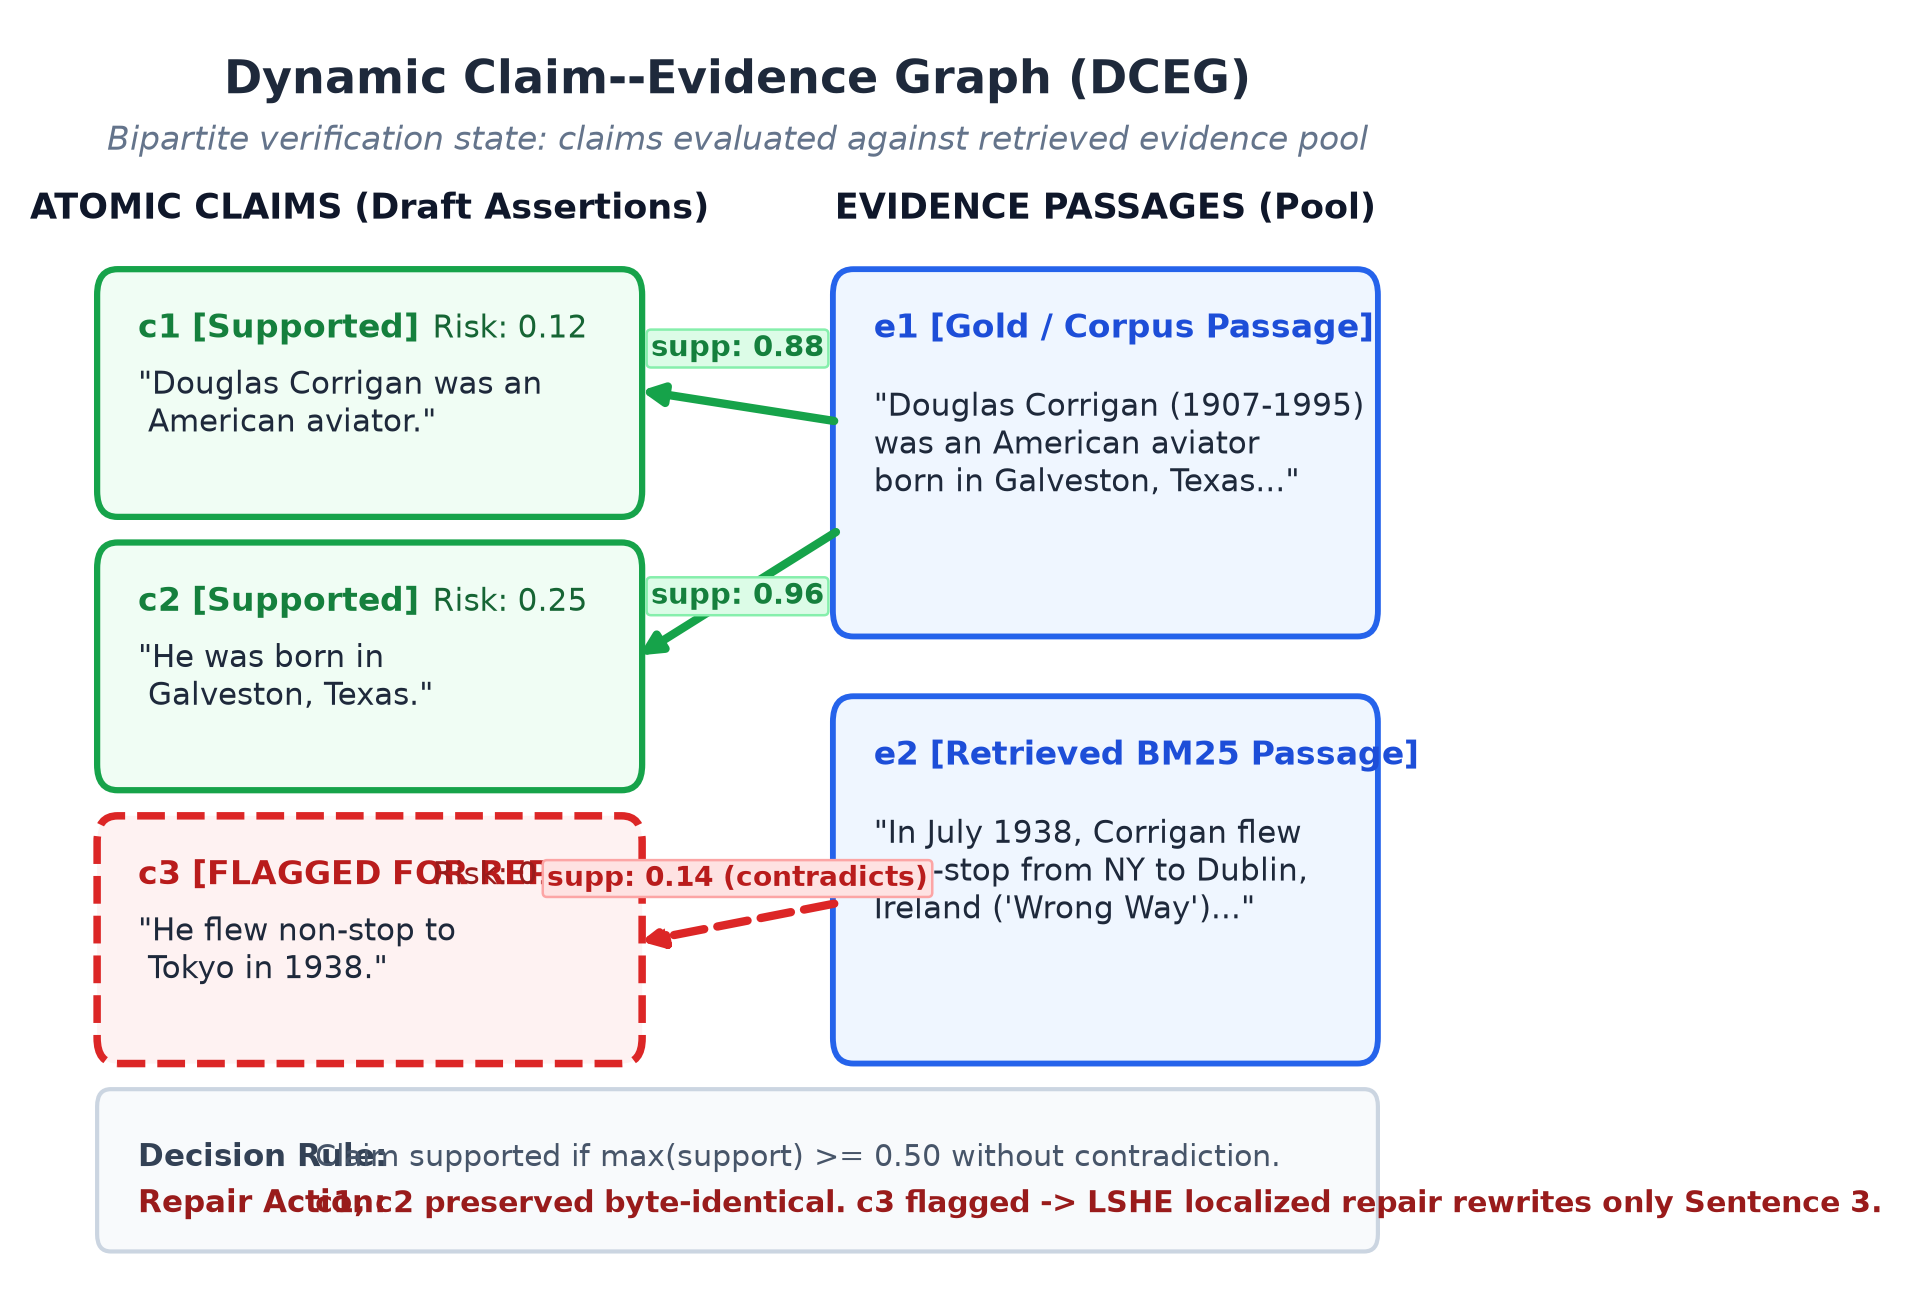
\includegraphics[width=\columnwidth]{figures/dceg_example.png}
\caption{Dynamic Claim--Evidence Graph (DCEG) exported by the prototype (\texttt{healgen/graph.py}). Bipartite state links atomic claims ($c_1, c_2, c_3$) to evidence passages ($e_1, e_2$) with NLI support scores. $c_1$ and $c_2$ meet the support threshold ($\ge 0.50$) and pass through untouched. $c_3$ receives low support ($0.14$, contradiction with Dublin flight) and is flagged for localized sentence repair.}
\label{fig:dceg}
\end{figure}

\paragraph{Step 6: Dynamic claim--evidence graph (\texttt{graph.py}).}
The system builds a bipartite graph linking all claims to available passages (Figure~\ref{fig:dceg}). A validated NLI judge scores each claim--evidence pair:
\begin{itemize}
  \item $e_1 \rightarrow c_1$: support = $0.88$ [Supported]
  \item $e_1 \rightarrow c_2$: support = $0.96$ [Supported]
  \item $e_2 \rightarrow c_3$: support = $0.14$ [Unsupported / Contradiction]
\end{itemize}
Claims $c_1$ and $c_2$ meet the threshold $\ge 0.50$, while $c_3$ lacks adequate support and is flagged for repair.

\paragraph{Step 7: Localized self-healing (\texttt{repair.py}).}
Rather than regenerating the whole response, the Localized Self-Healing Engine (LSHE) identifies the exact sentence containing $c_3$ (Sentence 3) via character offsets. Sentences 1 and 2 remain \textbf{100\% byte-identical}. Sentence 3 is regenerated using the retrieved passage $e_2$ in the prompt:
\begin{quote}
  \emph{``In July 1938, he flew non-stop from New York to Dublin, Ireland.''}
\end{quote}

\paragraph{Step 8: Confidence composition.}
The final answer is reassembled with statement-level reliability confidences ($0.88, 0.96, 0.85$). Downstream applications can display these confidences directly to users, ensuring full transparency.
